\begin {itemize}
\item Use Cases
\begin {itemize}
\item {addAuthorizationRestriction}\\
Adds an authorization restriction for a user role and a particular buzz space (implemented in code only, no functional way to test)
\begin {itemize}
\item Pre-conditions:\\
-an authorization restriction does not yet exist for the specified user role and buzz space (not implemented)\\
        -user has administrative rights (not implemented)\\

\item Post-conditions:\\
-authorization restriction must be persisted (not implemented)\\
\end {itemize}

\begin{figure}[h!]
  \centering
    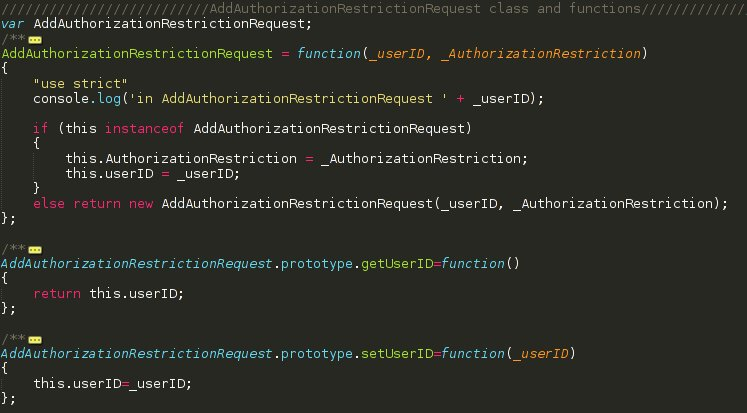
\includegraphics[width=0.85\textwidth]{buzzAuthorizationAddRestrictionCode}
    \caption{Add restriction}
\end{figure}


\item {isAuthorized}\\
Service used to determine which system services are available to the user. (implemented in code only, no functional way to test)
\begin {itemize}
\item Pre-conditions: \\
-buzz space is active (not implemented)\\ 
\end{itemize}

\begin{figure}[h!]
  \centering
    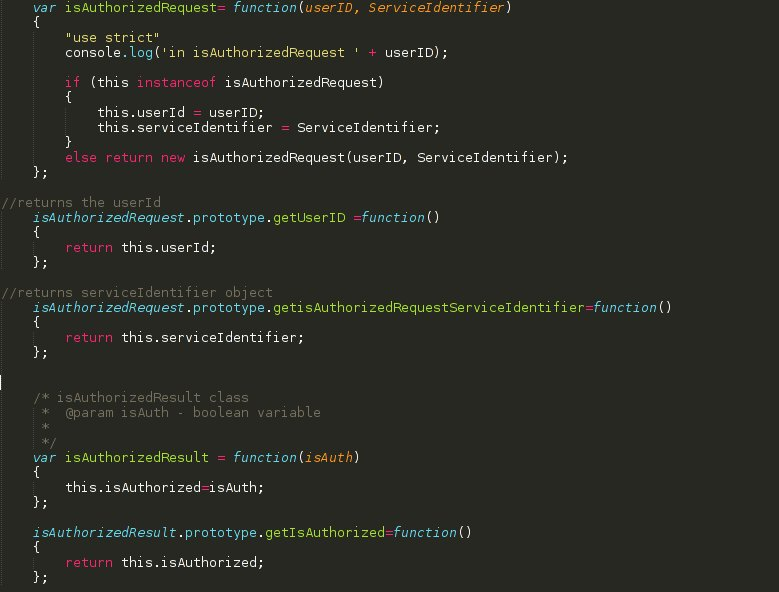
\includegraphics[width=0.85\textwidth]{buzzAuthorizationIsAuthorizedCode}
    \caption{isAuthorized}
\end{figure}

\item {removeAuthorizationRestriction}\\
Removes an authorization restriction for a user role and a particular buzz space (implemented in code only, no functional way to test)
\begin {itemize}
\item Pre-conditions: \\
-user has administrator role (not implemented)\\
        
\item Post-conditions: \\
  -authorization restriction for the user role must be removed from the buzz space (not implemented)
\end{itemize}

\begin{figure}[h!]
  \centering
    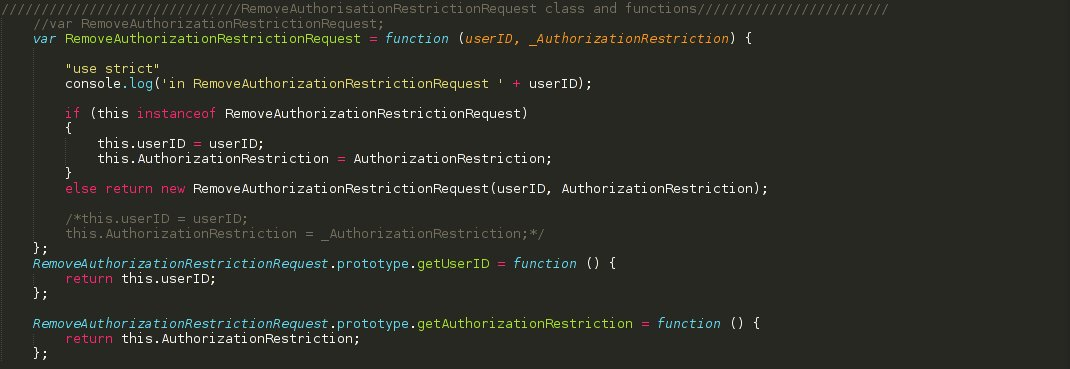
\includegraphics[width=0.85\textwidth]{buzzAuthorizationRemoveRestrictionCode}
    \caption{Remove restriction}
\end{figure}
 
\item{getAuthorizationRestrictions}
Returns authorization restrictions for a buzz space from the database (implemented in code only, no functional way to test) \\

\begin {itemize}
\item Pre-conditions: \\
-user has administrator role for space being queried (not implemented)\\
        -buzz space is active (not implemented)\\
         
\end{itemize}


\item {updateAuthorizationRestrictions}\\
Facilitates editing of authorization restrictions for a buzz space (implemented in code only, no functional way to test)
\begin {itemize}
\item Pre-conditions: \\
-user has administrator role for space being queried (not implemented)\\
        
\item Post-conditions: \\
  -new authorization restriction persisted to database (implemented in code only, no functional way to test)
\end{itemize}

\begin{figure}[h!]
  \centering
    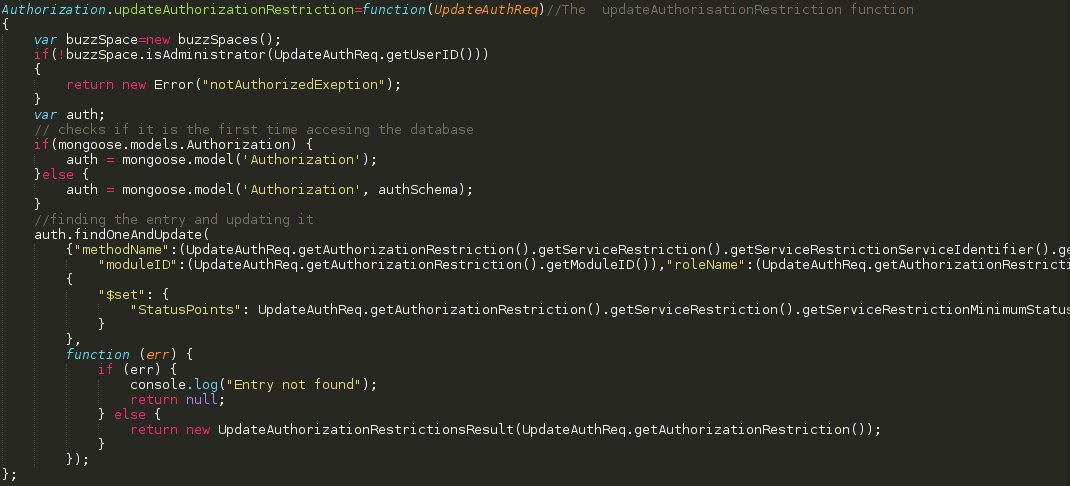
\includegraphics[width=0.85\textwidth]{buzzAuthorizationUpdateRestrictionsCode}
    \caption{Update restriction}
\end{figure}

\end{itemize}

\end{itemize}
